% Options for packages loaded elsewhere
\PassOptionsToPackage{unicode}{hyperref}
\PassOptionsToPackage{hyphens}{url}
\PassOptionsToPackage{dvipsnames,svgnames,x11names}{xcolor}
%
\documentclass[
  letterpaper,
  DIV=11,
  numbers=noendperiod]{scrartcl}

\usepackage{amsmath,amssymb}
\usepackage{iftex}
\ifPDFTeX
  \usepackage[T1]{fontenc}
  \usepackage[utf8]{inputenc}
  \usepackage{textcomp} % provide euro and other symbols
\else % if luatex or xetex
  \usepackage{unicode-math}
  \defaultfontfeatures{Scale=MatchLowercase}
  \defaultfontfeatures[\rmfamily]{Ligatures=TeX,Scale=1}
\fi
\usepackage{lmodern}
\ifPDFTeX\else  
    % xetex/luatex font selection
\fi
% Use upquote if available, for straight quotes in verbatim environments
\IfFileExists{upquote.sty}{\usepackage{upquote}}{}
\IfFileExists{microtype.sty}{% use microtype if available
  \usepackage[]{microtype}
  \UseMicrotypeSet[protrusion]{basicmath} % disable protrusion for tt fonts
}{}
\makeatletter
\@ifundefined{KOMAClassName}{% if non-KOMA class
  \IfFileExists{parskip.sty}{%
    \usepackage{parskip}
  }{% else
    \setlength{\parindent}{0pt}
    \setlength{\parskip}{6pt plus 2pt minus 1pt}}
}{% if KOMA class
  \KOMAoptions{parskip=half}}
\makeatother
\usepackage{xcolor}
\setlength{\emergencystretch}{3em} % prevent overfull lines
\setcounter{secnumdepth}{-\maxdimen} % remove section numbering
% Make \paragraph and \subparagraph free-standing
\ifx\paragraph\undefined\else
  \let\oldparagraph\paragraph
  \renewcommand{\paragraph}[1]{\oldparagraph{#1}\mbox{}}
\fi
\ifx\subparagraph\undefined\else
  \let\oldsubparagraph\subparagraph
  \renewcommand{\subparagraph}[1]{\oldsubparagraph{#1}\mbox{}}
\fi


\providecommand{\tightlist}{%
  \setlength{\itemsep}{0pt}\setlength{\parskip}{0pt}}\usepackage{longtable,booktabs,array}
\usepackage{calc} % for calculating minipage widths
% Correct order of tables after \paragraph or \subparagraph
\usepackage{etoolbox}
\makeatletter
\patchcmd\longtable{\par}{\if@noskipsec\mbox{}\fi\par}{}{}
\makeatother
% Allow footnotes in longtable head/foot
\IfFileExists{footnotehyper.sty}{\usepackage{footnotehyper}}{\usepackage{footnote}}
\makesavenoteenv{longtable}
\usepackage{graphicx}
\makeatletter
\def\maxwidth{\ifdim\Gin@nat@width>\linewidth\linewidth\else\Gin@nat@width\fi}
\def\maxheight{\ifdim\Gin@nat@height>\textheight\textheight\else\Gin@nat@height\fi}
\makeatother
% Scale images if necessary, so that they will not overflow the page
% margins by default, and it is still possible to overwrite the defaults
% using explicit options in \includegraphics[width, height, ...]{}
\setkeys{Gin}{width=\maxwidth,height=\maxheight,keepaspectratio}
% Set default figure placement to htbp
\makeatletter
\def\fps@figure{htbp}
\makeatother

\KOMAoption{captions}{tableheading}
\makeatletter
\makeatother
\makeatletter
\makeatother
\makeatletter
\@ifpackageloaded{caption}{}{\usepackage{caption}}
\AtBeginDocument{%
\ifdefined\contentsname
  \renewcommand*\contentsname{Table of contents}
\else
  \newcommand\contentsname{Table of contents}
\fi
\ifdefined\listfigurename
  \renewcommand*\listfigurename{List of Figures}
\else
  \newcommand\listfigurename{List of Figures}
\fi
\ifdefined\listtablename
  \renewcommand*\listtablename{List of Tables}
\else
  \newcommand\listtablename{List of Tables}
\fi
\ifdefined\figurename
  \renewcommand*\figurename{Figure}
\else
  \newcommand\figurename{Figure}
\fi
\ifdefined\tablename
  \renewcommand*\tablename{Table}
\else
  \newcommand\tablename{Table}
\fi
}
\@ifpackageloaded{float}{}{\usepackage{float}}
\floatstyle{ruled}
\@ifundefined{c@chapter}{\newfloat{codelisting}{h}{lop}}{\newfloat{codelisting}{h}{lop}[chapter]}
\floatname{codelisting}{Listing}
\newcommand*\listoflistings{\listof{codelisting}{List of Listings}}
\makeatother
\makeatletter
\@ifpackageloaded{caption}{}{\usepackage{caption}}
\@ifpackageloaded{subcaption}{}{\usepackage{subcaption}}
\makeatother
\makeatletter
\@ifpackageloaded{tcolorbox}{}{\usepackage[skins,breakable]{tcolorbox}}
\makeatother
\makeatletter
\@ifundefined{shadecolor}{\definecolor{shadecolor}{rgb}{.97, .97, .97}}
\makeatother
\makeatletter
\makeatother
\makeatletter
\makeatother
\ifLuaTeX
  \usepackage{selnolig}  % disable illegal ligatures
\fi
\IfFileExists{bookmark.sty}{\usepackage{bookmark}}{\usepackage{hyperref}}
\IfFileExists{xurl.sty}{\usepackage{xurl}}{} % add URL line breaks if available
\urlstyle{same} % disable monospaced font for URLs
\hypersetup{
  pdftitle={HW 01: Data Entry},
  colorlinks=true,
  linkcolor={blue},
  filecolor={Maroon},
  citecolor={Blue},
  urlcolor={Blue},
  pdfcreator={LaTeX via pandoc}}

\title{HW 01: Data Entry}
\usepackage{etoolbox}
\makeatletter
\providecommand{\subtitle}[1]{% add subtitle to \maketitle
  \apptocmd{\@title}{\par {\large #1 \par}}{}{}
}
\makeatother
\subtitle{Recording data to maintain your sanity.}
\author{}
\date{}

\begin{document}
\maketitle
\ifdefined\Shaded\renewenvironment{Shaded}{\begin{tcolorbox}[enhanced, borderline west={3pt}{0pt}{shadecolor}, sharp corners, interior hidden, boxrule=0pt, frame hidden, breakable]}{\end{tcolorbox}}\fi

\hypertarget{assignment-overview}{%
\section{Assignment Overview}\label{assignment-overview}}

Although you will be working with previously collected data, it is
important to understand what data looks like as well as how it is coded
and entered into a spreadsheet or dataset for analysis. This can help
you identify and avoid problems later when reading data into an analysis
software program. For example if you mix letters and numbers in the same
cell, the variable will be treated as character not numeric.

\hypertarget{instructions}{%
\section{Instructions}\label{instructions}}

Preparation: Read
\href{https://tidyr.tidyverse.org/articles/tidy-data.html\#tidying}{Tidy
data principles} by Wickham, Vaughan, and Girlich.

There are three pieces to this assignment.

\begin{enumerate}
\def\labelenumi{\arabic{enumi}.}
\tightlist
\item
  Entering raw data into a spreadsheet.
\item
  Creating a codebook
\item
  Importing the data into R
\end{enumerate}

Using the \href{hw/medical-records.pdf}{PDF copies of medical records}
for 5 patients seeking treatment in a hospital emergency room you are
going to do data entry and create a codebook.

\hypertarget{submission-instructions}{%
\subsection{Submission Instructions}\label{submission-instructions}}

You will enter data and create your codebook directly in Google Sheets,
and submit screenshots to Canvas.

\begin{itemize}
\tightlist
\item
  Start a new Google spreadsheet in the \textbf{01 Data Entry} folder in
  our shared Google Drive.
\item
  Name this file \texttt{medrecords\_userid} where \emph{userid} is your
  chico state user id.
\item
  Create and name the following worksheets: \texttt{data},
  \texttt{codebook}, \texttt{import}.
\end{itemize}

\begin{center}\rule{0.5\linewidth}{0.5pt}\end{center}

\hypertarget{assignment}{%
\section{Assignment}\label{assignment}}

\hypertarget{data-entry}{%
\subsection{1. Data Entry}\label{data-entry}}

\begin{enumerate}
\def\labelenumi{\arabic{enumi}.}
\tightlist
\item
  Select 4 variables recorded on the medical forms

  \begin{itemize}
  \tightlist
  \item
    one should be a unique identifier, at least one should be a
    quantitative variable and at least one should be a categorical
    variable. (Ref PMA6 Ch2)
  \end{itemize}
\item
  Select a brief name for each variable - write this in the first row

  \begin{itemize}
  \tightlist
  \item
    Use good variable naming conventions:

    \begin{itemize}
    \tightlist
    \item
      short
    \item
      no special characters
    \item
      no spaces
    \item
      doesn't start with a number
    \end{itemize}
  \end{itemize}
\item
  Determine what range of values is needed for recording each variable
\item
  Enter the data for each patient, one patient per row.
\item
  If data is missing for a particular value, leave the cell blank.
\end{enumerate}

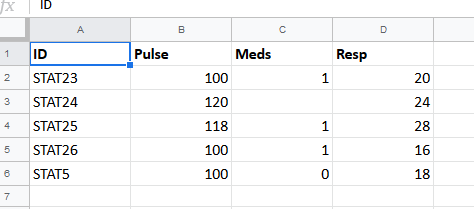
\includegraphics{images/hw1_data.png}

Recall the \emph{tidy data principles} state to put one observation per
row, and one variable (characteristic) per column.

\hypertarget{codebook-creation}{%
\subsection{2. Codebook Creation}\label{codebook-creation}}

In a separate worksheet list the variable names, labels, data types, and
response code or ranges in separate columns (4 columns total).

An example of what this should look like is below. (With the exception
of the red error)

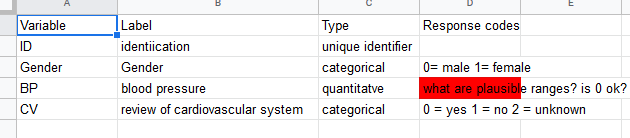
\includegraphics{images/hw1_codebook.png}

\hypertarget{data-import}{%
\subsection{3. Data Import}\label{data-import}}

\begin{enumerate}
\def\labelenumi{\arabic{enumi}.}
\tightlist
\item
  Export your file to your hard drive as a Comma Separated Value
  (\texttt{*.csv}).

  \begin{itemize}
  \tightlist
  \item
    If it asks you, only save the\texttt{data} worksheet.
  \end{itemize}
\item
  Import this data into R.

  \begin{itemize}
  \tightlist
  \item
    Code is fine if you already know how. Point and click is also fine
    for now.
  \item
    \href{https://support.posit.co/hc/en-us/articles/218611977-Importing-Data-with-the-RStudio-IDE}{Point
    and click instructions}
  \item
    Code examples from {[}R for data
    science{]}{]}(https://r4ds.hadley.nz/data-import{]} and
    \href{https://www.statology.org/import-csv-into-r/}{Statology}
  \end{itemize}
\item
  Note and record any problems that you noticed and/or had to fix at the
  bottom of your \texttt{codebook} worksheet.

  \begin{itemize}
  \tightlist
  \item
    Does your data file look like your spreadsheet?
  \item
    Did you have to specify missing values in any specific way?
  \end{itemize}
\item
  Show that it worked by taking a screenshot of BOTH the code, and the
  view of the data.

  \begin{itemize}
  \tightlist
  \item
    Paste these images into your \texttt{import} tab.
  \end{itemize}
\end{enumerate}

\hypertarget{examples-of-import-code}{%
\subsubsection{Examples of import code}\label{examples-of-import-code}}

\begin{figure}

{\centering 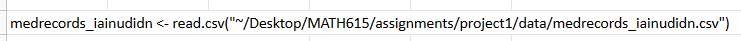
\includegraphics{images/hw1_r_code.png}

}

\caption{Example R code}

\end{figure}



\end{document}
